\documentclass[1p]{elsarticle_modified}
%\bibliographystyle{elsarticle-num}

%\usepackage[colorlinks]{hyperref}
%\usepackage{abbrmath_seonhwa} %\Abb, \Ascr, \Acal ,\Abf, \Afrak
\usepackage{amsfonts}
\usepackage{amssymb}
\usepackage{amsmath}
\usepackage{amsthm}
\usepackage{scalefnt}
\usepackage{amsbsy}
\usepackage{kotex}
\usepackage{caption}
\usepackage{subfig}
\usepackage{color}
\usepackage{graphicx}
\usepackage{xcolor} %% white, black, red, green, blue, cyan, magenta, yellow
\usepackage{float}
\usepackage{setspace}
\usepackage{hyperref}

\usepackage{tikz}
\usetikzlibrary{arrows}

\usepackage{multirow}
\usepackage{array} % fixed length table
\usepackage{hhline}

%%%%%%%%%%%%%%%%%%%%%
\makeatletter
\renewcommand*\env@matrix[1][\arraystretch]{%
	\edef\arraystretch{#1}%
	\hskip -\arraycolsep
	\let\@ifnextchar\new@ifnextchar
	\array{*\c@MaxMatrixCols c}}
\makeatother %https://tex.stackexchange.com/questions/14071/how-can-i-increase-the-line-spacing-in-a-matrix
%%%%%%%%%%%%%%%

\usepackage[normalem]{ulem}

\newcommand{\msout}[1]{\ifmmode\text{\sout{\ensuremath{#1}}}\else\sout{#1}\fi}
%SOURCE: \msout is \stkout macro in https://tex.stackexchange.com/questions/20609/strikeout-in-math-mode

\newcommand{\cancel}[1]{
	\ifmmode
	{\color{red}\msout{#1}}
	\else
	{\color{red}\sout{#1}}
	\fi
}

\newcommand{\add}[1]{
	{\color{blue}\uwave{#1}}
}

\newcommand{\replace}[2]{
	\ifmmode
	{\color{red}\msout{#1}}{\color{blue}\uwave{#2}}
	\else
	{\color{red}\sout{#1}}{\color{blue}\uwave{#2}}
	\fi
}

\newcommand{\Sol}{\mathcal{S}} %segment
\newcommand{\D}{D} %diagram
\newcommand{\A}{\mathcal{A}} %arc


%%%%%%%%%%%%%%%%%%%%%%%%%%%%%5 test

\def\sl{\operatorname{\textup{SL}}(2,\Cbb)}
\def\psl{\operatorname{\textup{PSL}}(2,\Cbb)}
\def\quan{\mkern 1mu \triangleright \mkern 1mu}

\theoremstyle{definition}
\newtheorem{thm}{Theorem}[section]
\newtheorem{prop}[thm]{Proposition}
\newtheorem{lem}[thm]{Lemma}
\newtheorem{ques}[thm]{Question}
\newtheorem{cor}[thm]{Corollary}
\newtheorem{defn}[thm]{Definition}
\newtheorem{exam}[thm]{Example}
\newtheorem{rmk}[thm]{Remark}
\newtheorem{alg}[thm]{Algorithm}

\newcommand{\I}{\sqrt{-1}}
\begin{document}

%\begin{frontmatter}
%
%\title{Boundary parabolic representations of knots up to 8 crossings}
%
%%% Group authors per affiliation:
%\author{Yunhi Cho} 
%\address{Department of Mathematics, University of Seoul, Seoul, Korea}
%\ead{yhcho@uos.ac.kr}
%
%
%\author{Seonhwa Kim} %\fnref{s_kim}}
%\address{Center for Geometry and Physics, Institute for Basic Science, Pohang, 37673, Korea}
%\ead{ryeona17@ibs.re.kr}
%
%\author{Hyuk Kim}
%\address{Department of Mathematical Sciences, Seoul National University, Seoul 08826, Korea}
%\ead{hyukkim@snu.ac.kr}
%
%\author{Seokbeom Yoon}
%\address{Department of Mathematical Sciences, Seoul National University, Seoul, 08826,  Korea}
%\ead{sbyoon15@snu.ac.kr}
%
%\begin{abstract}
%We find all boundary parabolic representation of knots up to 8 crossings.
%
%\end{abstract}
%\begin{keyword}
%    \MSC[2010] 57M25 
%\end{keyword}
%
%\end{frontmatter}

%\linenumbers
%\tableofcontents
%
\newcommand\colored[1]{\textcolor{white}{\rule[-0.35ex]{0.8em}{1.4ex}}\kern-0.8em\color{red} #1}%
%\newcommand\colored[1]{\textcolor{white}{ #1}\kern-2.17ex	\textcolor{white}{ #1}\kern-1.81ex	\textcolor{white}{ #1}\kern-2.15ex\color{red}#1	}

{\Large $\underline{12a_{0450}~(K12a_{0450})}$}

\setlength{\tabcolsep}{10pt}
\renewcommand{\arraystretch}{1.6}
\vspace{1cm}\begin{tabular}{m{100pt}>{\centering\arraybackslash}m{274pt}}
\multirow{5}{120pt}{
	\centering
	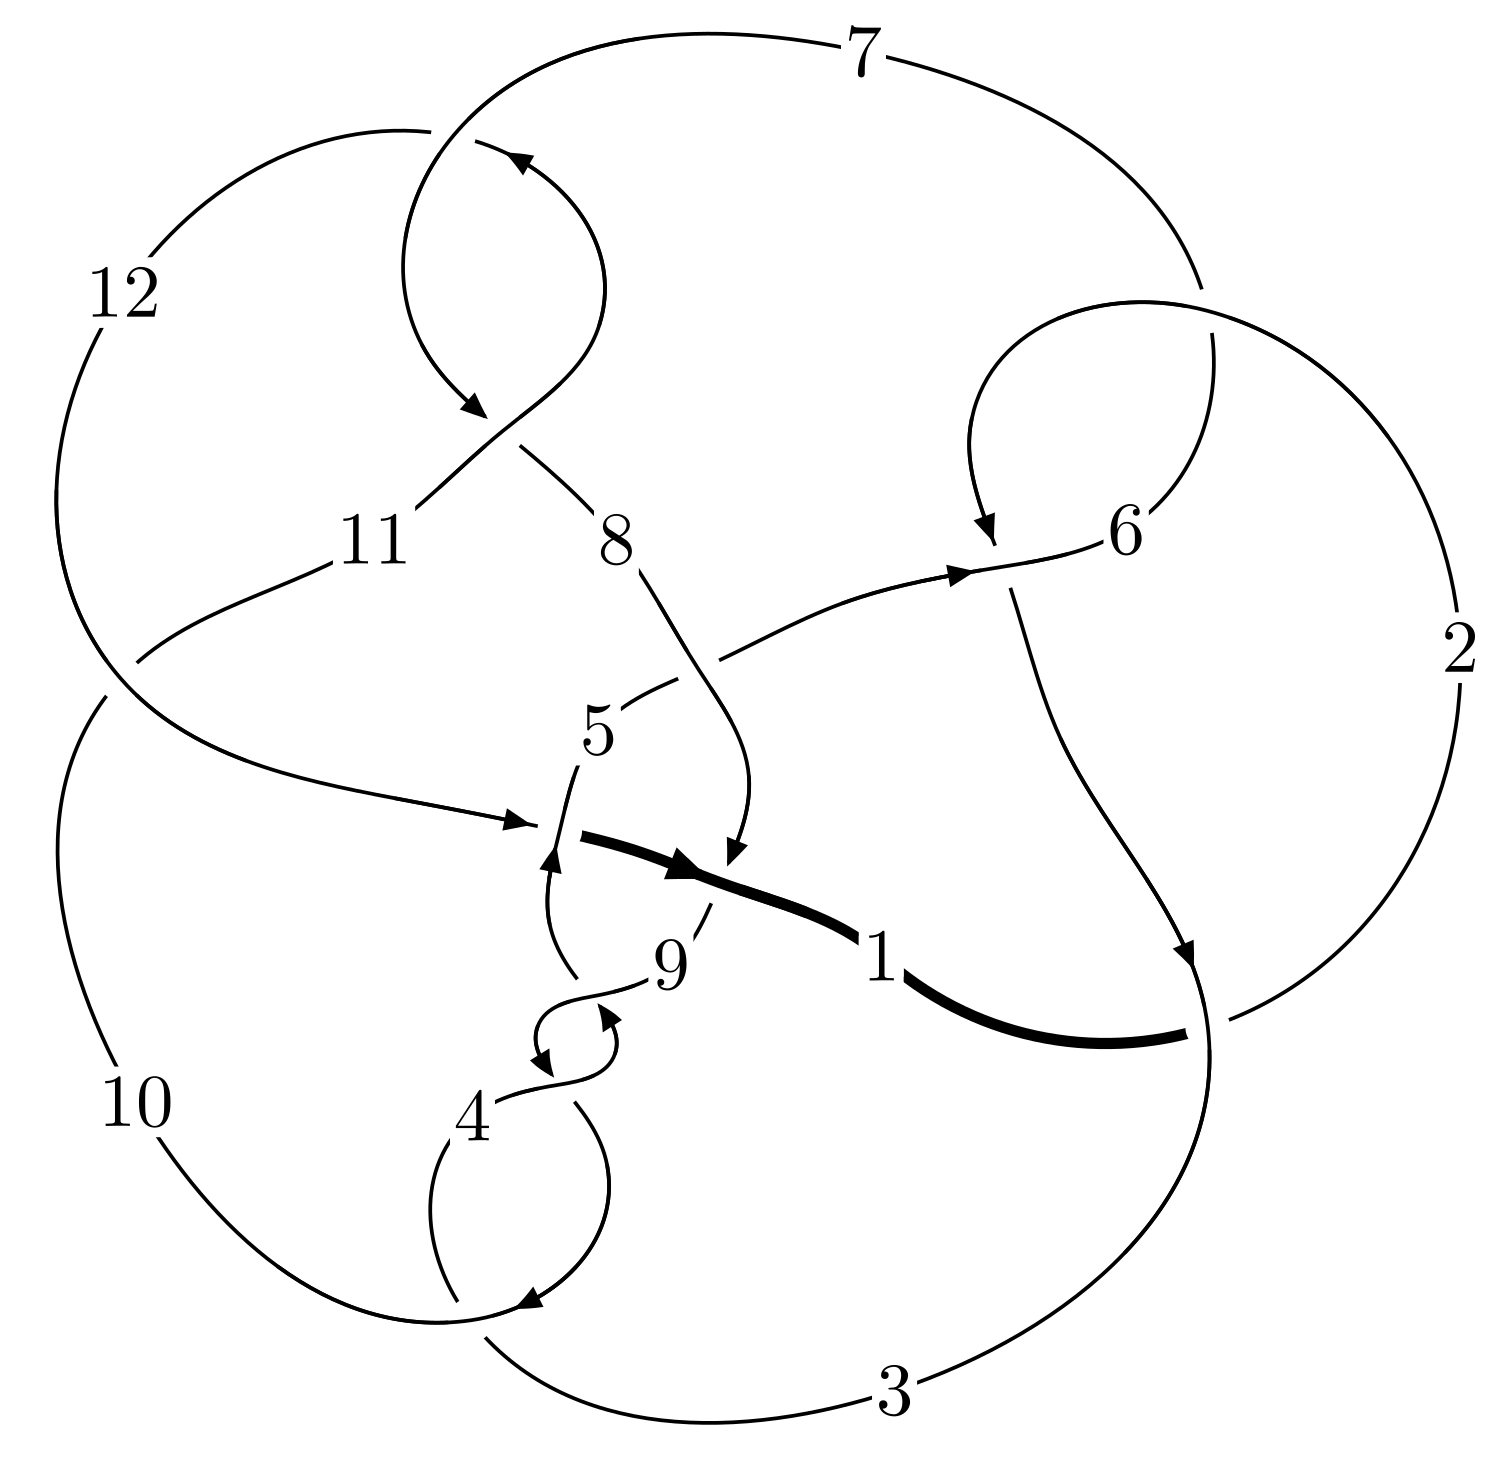
\includegraphics[width=112pt]{../../../GIT/diagram.site/Diagrams/png/1251_12a_0450.png}\\
\ \ \ A knot diagram\footnotemark}&
\allowdisplaybreaks
\textbf{Linearized knot diagam} \\
\cline{2-2}
 &
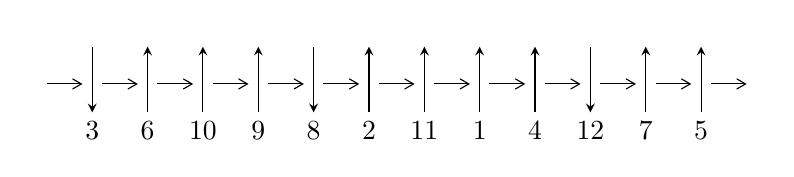
\begin{tikzpicture}[x=20pt, y=17pt]
	% nodes
	\node (C0) at (0, 0) {};
	\node (C1) at (1, 0) {};
	\node (C1U) at (1, +1) {};
	\node (C1D) at (1, -1) {3};

	\node (C2) at (2, 0) {};
	\node (C2U) at (2, +1) {};
	\node (C2D) at (2, -1) {6};

	\node (C3) at (3, 0) {};
	\node (C3U) at (3, +1) {};
	\node (C3D) at (3, -1) {10};

	\node (C4) at (4, 0) {};
	\node (C4U) at (4, +1) {};
	\node (C4D) at (4, -1) {9};

	\node (C5) at (5, 0) {};
	\node (C5U) at (5, +1) {};
	\node (C5D) at (5, -1) {8};

	\node (C6) at (6, 0) {};
	\node (C6U) at (6, +1) {};
	\node (C6D) at (6, -1) {2};

	\node (C7) at (7, 0) {};
	\node (C7U) at (7, +1) {};
	\node (C7D) at (7, -1) {11};

	\node (C8) at (8, 0) {};
	\node (C8U) at (8, +1) {};
	\node (C8D) at (8, -1) {1};

	\node (C9) at (9, 0) {};
	\node (C9U) at (9, +1) {};
	\node (C9D) at (9, -1) {4};

	\node (C10) at (10, 0) {};
	\node (C10U) at (10, +1) {};
	\node (C10D) at (10, -1) {12};

	\node (C11) at (11, 0) {};
	\node (C11U) at (11, +1) {};
	\node (C11D) at (11, -1) {7};

	\node (C12) at (12, 0) {};
	\node (C12U) at (12, +1) {};
	\node (C12D) at (12, -1) {5};
	\node (C13) at (13, 0) {};

	% arrows
	\draw[->,>={angle 60}]
	(C0) edge (C1) (C1) edge (C2) (C2) edge (C3) (C3) edge (C4) (C4) edge (C5) (C5) edge (C6) (C6) edge (C7) (C7) edge (C8) (C8) edge (C9) (C9) edge (C10) (C10) edge (C11) (C11) edge (C12) (C12) edge (C13) ;	\draw[->,>=stealth]
	(C1U) edge (C1D) (C2D) edge (C2U) (C3D) edge (C3U) (C4D) edge (C4U) (C5U) edge (C5D) (C6D) edge (C6U) (C7D) edge (C7U) (C8D) edge (C8U) (C9D) edge (C9U) (C10U) edge (C10D) (C11D) edge (C11U) (C12D) edge (C12U) ;
	\end{tikzpicture} \\
\hhline{~~} \\& 
\textbf{Solving Sequence} \\ \cline{2-2} 
 &
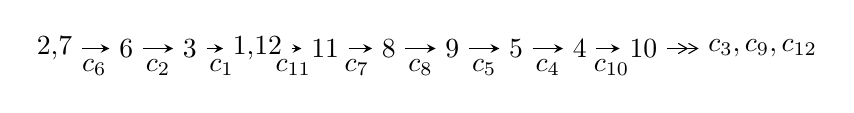
\begin{tikzpicture}[x=23pt, y=7pt]
	% node
	\node (A0) at (-1/8, 0) {2,7};
	\node (A1) at (1, 0) {6};
	\node (A2) at (2, 0) {3};
	\node (A3) at (49/16, 0) {1,12};
	\node (A4) at (33/8, 0) {11};
	\node (A5) at (41/8, 0) {8};
	\node (A6) at (49/8, 0) {9};
	\node (A7) at (57/8, 0) {5};
	\node (A8) at (65/8, 0) {4};
	\node (A9) at (73/8, 0) {10};
	\node (C1) at (1/2, -1) {$c_{6}$};
	\node (C2) at (3/2, -1) {$c_{2}$};
	\node (C3) at (5/2, -1) {$c_{1}$};
	\node (C4) at (29/8, -1) {$c_{11}$};
	\node (C5) at (37/8, -1) {$c_{7}$};
	\node (C6) at (45/8, -1) {$c_{8}$};
	\node (C7) at (53/8, -1) {$c_{5}$};
	\node (C8) at (61/8, -1) {$c_{4}$};
	\node (C9) at (69/8, -1) {$c_{10}$};
	\node (A10) at (11, 0) {$c_{3},c_{9},c_{12}$};

	% edge
	\draw[->,>=stealth]	
	(A0) edge (A1) (A1) edge (A2) (A2) edge (A3) (A3) edge (A4) (A4) edge (A5) (A5) edge (A6) (A6) edge (A7) (A7) edge (A8) (A8) edge (A9) ;
	\draw[->>,>={angle 60}]	
	(A9) edge (A10);
\end{tikzpicture} \\ 

\end{tabular} \\

\footnotetext{
The image of knot diagram is generated by the software ``\textbf{Draw programme}" developed by Andrew Bartholomew(\url{http://www.layer8.co.uk/maths/draw/index.htm\#Running-draw}), where we modified some parts for our purpose(\url{https://github.com/CATsTAILs/LinksPainter}).
}\phantom \\ \newline 
\centering \textbf{Ideals for irreducible components\footnotemark of $X_{\text{par}}$} 
 
\begin{align*}
I^u_{1}&=\langle 
b- u,\;-11204011 u^{28}+11782800 u^{27}+\cdots+11150225 a+3596564,\;u^{29}- u^{28}+\cdots+u-1\rangle \\
I^u_{2}&=\langle 
-1.58760\times10^{230} u^{101}-4.36695\times10^{230} u^{100}+\cdots+1.89430\times10^{230} b+1.72802\times10^{231},\\
\phantom{I^u_{2}}&\phantom{= \langle  }1.44256\times10^{231} u^{101}+3.32780\times10^{231} u^{100}+\cdots+7.00892\times10^{231} a+5.69101\times10^{232},\\
\phantom{I^u_{2}}&\phantom{= \langle  }u^{102}+2 u^{101}+\cdots+355 u+37\rangle \\
I^u_{3}&=\langle 
b+u,\\
\phantom{I^u_{3}}&\phantom{= \langle  }4 u^{13}+5 u^{12}+15 u^{11}+14 u^{10}+31 u^9+27 u^8+41 u^7+30 u^6+36 u^5+25 u^4+25 u^3+13 u^2+a+9 u+5,\\
\phantom{I^u_{3}}&\phantom{= \langle  }u^{14}+u^{13}+4 u^{12}+3 u^{11}+9 u^{10}+6 u^9+13 u^8+7 u^7+13 u^6+6 u^5+10 u^4+3 u^3+5 u^2+u+1\rangle \\
I^u_{4}&=\langle 
- u^{13}- u^{12}-4 u^{11}-3 u^{10}-9 u^9-6 u^8-14 u^7-7 u^6-14 u^5-6 u^4-9 u^3-3 u^2+b-4 u-1,\\
\phantom{I^u_{4}}&\phantom{= \langle  }3 u^{13}+4 u^{12}+11 u^{11}+11 u^{10}+22 u^9+21 u^8+31 u^7+24 u^6+24 u^5+20 u^4+10 u^3+9 u^2+a+4 u+3,\\
\phantom{I^u_{4}}&\phantom{= \langle  }u^{14}+u^{13}+4 u^{12}+3 u^{11}+9 u^{10}+6 u^9+14 u^8+7 u^7+14 u^6+6 u^5+9 u^4+3 u^3+4 u^2+u+1\rangle \\
\\
\end{align*}
\raggedright * 4 irreducible components of $\dim_{\mathbb{C}}=0$, with total 159 representations.\\
\footnotetext{All coefficients of polynomials are rational numbers. But the coefficients are sometimes approximated in decimal forms when there is not enough margin.}
\newpage
\renewcommand{\arraystretch}{1}
\centering \section*{I. $I^u_{1}= \langle b- u,\;-1.12\times10^{7} u^{28}+1.18\times10^{7} u^{27}+\cdots+1.12\times10^{7} a+3.60\times10^{6},\;u^{29}- u^{28}+\cdots+u-1 \rangle$}
\flushleft \textbf{(i) Arc colorings}\\
\begin{tabular}{m{7pt} m{180pt} m{7pt} m{180pt} }
\flushright $a_{2}=$&$\begin{pmatrix}0\\u\end{pmatrix}$ \\
\flushright $a_{7}=$&$\begin{pmatrix}1\\0\end{pmatrix}$ \\
\flushright $a_{6}=$&$\begin{pmatrix}1\\u^2\end{pmatrix}$ \\
\flushright $a_{3}=$&$\begin{pmatrix}u\\u^3+u\end{pmatrix}$ \\
\flushright $a_{1}=$&$\begin{pmatrix}u^3\\u^5+u^3+u\end{pmatrix}$ \\
\flushright $a_{12}=$&$\begin{pmatrix}1.00482 u^{28}-1.05673 u^{27}+\cdots-1.71703 u-0.322555\\u\end{pmatrix}$ \\
\flushright $a_{11}=$&$\begin{pmatrix}1.00482 u^{28}-1.05673 u^{27}+\cdots-2.71703 u-0.322555\\u\end{pmatrix}$ \\
\flushright $a_{8}=$&$\begin{pmatrix}0.0519083 u^{28}-0.150688 u^{27}+\cdots+1.32738 u-0.00482376\\- u^2\end{pmatrix}$ \\
\flushright $a_{9}=$&$\begin{pmatrix}-0.189436 u^{28}+0.263701 u^{27}+\cdots+1.76119 u-0.259466\\0.108962 u^{28}-0.0707161 u^{27}+\cdots-0.422843 u+0.0385933\end{pmatrix}$ \\
\flushright $a_{5}=$&$\begin{pmatrix}0.354849 u^{28}-0.895361 u^{27}+\cdots+0.459547 u+0.601333\\-0.147097 u^{28}+0.813257 u^{27}+\cdots+0.521680 u-0.644748\end{pmatrix}$ \\
\flushright $a_{4}=$&$\begin{pmatrix}0.00618741 u^{28}+0.549901 u^{27}+\cdots+0.308783 u+0.152467\\-0.113039 u^{28}+0.353098 u^{27}+\cdots+1.44615 u-0.413071\end{pmatrix}$ \\
\flushright $a_{10}=$&$\begin{pmatrix}1.10360 u^{28}-1.27858 u^{27}+\cdots-1.66030 u-0.374464\\u^3+u\end{pmatrix}$\\&\end{tabular}
\flushleft \textbf{(ii) Obstruction class $= -1$}\\~\\
\flushleft \textbf{(iii) Cusp Shapes $= \frac{32073842}{11150225} u^{28}-\frac{607928}{446009} u^{27}+\cdots+\frac{2213155}{446009} u+\frac{88659642}{11150225}$}\\~\\
\newpage\renewcommand{\arraystretch}{1}
\flushleft \textbf{(iv) u-Polynomials at the component}\newline \\
\begin{tabular}{m{50pt}|m{274pt}}
Crossings & \hspace{64pt}u-Polynomials at each crossing \\
\hline $$\begin{aligned}c_{1},c_{10}\end{aligned}$$&$\begin{aligned}
&u^{29}+15 u^{28}+\cdots+7 u-1
\end{aligned}$\\
\hline $$\begin{aligned}c_{2},c_{6},c_{7}\\c_{11}\end{aligned}$$&$\begin{aligned}
&u^{29}- u^{28}+\cdots+u-1
\end{aligned}$\\
\hline $$\begin{aligned}c_{3},c_{4},c_{9}\end{aligned}$$&$\begin{aligned}
&u^{29}-11 u^{28}+\cdots+344 u-32
\end{aligned}$\\
\hline $$\begin{aligned}c_{5}\end{aligned}$$&$\begin{aligned}
&u^{29}-25 u^{28}+\cdots+30720 u-2048
\end{aligned}$\\
\hline $$\begin{aligned}c_{8},c_{12}\end{aligned}$$&$\begin{aligned}
&u^{29}+7 u^{27}+\cdots-2 u-1
\end{aligned}$\\
\hline
\end{tabular}\\~\\
\newpage\renewcommand{\arraystretch}{1}
\flushleft \textbf{(v) Riley Polynomials at the component}\newline \\
\begin{tabular}{m{50pt}|m{274pt}}
Crossings & \hspace{64pt}Riley Polynomials at each crossing \\
\hline $$\begin{aligned}c_{1},c_{10}\end{aligned}$$&$\begin{aligned}
&y^{29}+7 y^{28}+\cdots+111 y-1
\end{aligned}$\\
\hline $$\begin{aligned}c_{2},c_{6},c_{7}\\c_{11}\end{aligned}$$&$\begin{aligned}
&y^{29}+15 y^{28}+\cdots+7 y-1
\end{aligned}$\\
\hline $$\begin{aligned}c_{3},c_{4},c_{9}\end{aligned}$$&$\begin{aligned}
&y^{29}+25 y^{28}+\cdots-1728 y-1024
\end{aligned}$\\
\hline $$\begin{aligned}c_{5}\end{aligned}$$&$\begin{aligned}
&y^{29}-3 y^{28}+\cdots+85983232 y-4194304
\end{aligned}$\\
\hline $$\begin{aligned}c_{8},c_{12}\end{aligned}$$&$\begin{aligned}
&y^{29}+14 y^{28}+\cdots-30 y-1
\end{aligned}$\\
\hline
\end{tabular}\\~\\
\newpage\flushleft \textbf{(vi) Complex Volumes and Cusp Shapes}
$$\begin{array}{c|c|c}  
\text{Solutions to }I^u_{1}& \I (\text{vol} + \sqrt{-1}CS) & \text{Cusp shape}\\
 \hline 
\begin{aligned}
u &= -0.823702 + 0.553499 I \\
a &= -1.386270 + 0.264015 I \\
b &= -0.823702 + 0.553499 I\end{aligned}
 & \phantom{-}4.15742 + 2.94610 I & \phantom{-}10.44832 - 2.08399 I \\ \hline\begin{aligned}
u &= -0.823702 - 0.553499 I \\
a &= -1.386270 - 0.264015 I \\
b &= -0.823702 - 0.553499 I\end{aligned}
 & \phantom{-}4.15742 - 2.94610 I & \phantom{-}10.44832 + 2.08399 I \\ \hline\begin{aligned}
u &= \phantom{-}0.909923 + 0.492711 I \\
a &= \phantom{-}1.55550 + 0.08106 I \\
b &= \phantom{-}0.909923 + 0.492711 I\end{aligned}
 & -1.63366 - 6.77137 I & \phantom{-}6.32659 + 2.86609 I \\ \hline\begin{aligned}
u &= \phantom{-}0.909923 - 0.492711 I \\
a &= \phantom{-}1.55550 - 0.08106 I \\
b &= \phantom{-}0.909923 - 0.492711 I\end{aligned}
 & -1.63366 + 6.77137 I & \phantom{-}6.32659 - 2.86609 I \\ \hline\begin{aligned}
u &= -0.139705 + 1.052750 I \\
a &= -0.94818 - 1.53693 I \\
b &= -0.139705 + 1.052750 I\end{aligned}
 & -5.81423 + 0.14287 I & -5.03844 - 0.22076 I \\ \hline\begin{aligned}
u &= -0.139705 - 1.052750 I \\
a &= -0.94818 + 1.53693 I \\
b &= -0.139705 - 1.052750 I\end{aligned}
 & -5.81423 - 0.14287 I & -5.03844 + 0.22076 I \\ \hline\begin{aligned}
u &= \phantom{-}0.501294 + 0.940692 I \\
a &= \phantom{-}3.02556 - 0.44481 I \\
b &= \phantom{-}0.501294 + 0.940692 I\end{aligned}
 & -1.91483 + 3.97058 I & \phantom{-}1.30591 - 5.30743 I \\ \hline\begin{aligned}
u &= \phantom{-}0.501294 - 0.940692 I \\
a &= \phantom{-}3.02556 + 0.44481 I \\
b &= \phantom{-}0.501294 - 0.940692 I\end{aligned}
 & -1.91483 - 3.97058 I & \phantom{-}1.30591 + 5.30743 I \\ \hline\begin{aligned}
u &= \phantom{-}0.688832 + 0.611331 I \\
a &= \phantom{-}1.036710 + 0.591577 I \\
b &= \phantom{-}0.688832 + 0.611331 I\end{aligned}
 & \phantom{-}2.69727 + 1.72831 I & \phantom{-}8.88157 - 2.20446 I \\ \hline\begin{aligned}
u &= \phantom{-}0.688832 - 0.611331 I \\
a &= \phantom{-}1.036710 - 0.591577 I \\
b &= \phantom{-}0.688832 - 0.611331 I\end{aligned}
 & \phantom{-}2.69727 - 1.72831 I & \phantom{-}8.88157 + 2.20446 I\\
 \hline 
 \end{array}$$\newpage$$\begin{array}{c|c|c}  
\text{Solutions to }I^u_{1}& \I (\text{vol} + \sqrt{-1}CS) & \text{Cusp shape}\\
 \hline 
\begin{aligned}
u &= -0.381004 + 0.827261 I \\
a &= -3.27823 - 1.66424 I \\
b &= -0.381004 + 0.827261 I\end{aligned}
 & -5.43501 + 1.14701 I & -0.01474 + 3.75777 I \\ \hline\begin{aligned}
u &= -0.381004 - 0.827261 I \\
a &= -3.27823 + 1.66424 I \\
b &= -0.381004 - 0.827261 I\end{aligned}
 & -5.43501 - 1.14701 I & -0.01474 - 3.75777 I \\ \hline\begin{aligned}
u &= \phantom{-}0.200189 + 0.870048 I \\
a &= -0.372681 - 0.947305 I \\
b &= \phantom{-}0.200189 + 0.870048 I\end{aligned}
 & -1.79658 + 2.03837 I & \phantom{-}4.94429 - 3.28871 I \\ \hline\begin{aligned}
u &= \phantom{-}0.200189 - 0.870048 I \\
a &= -0.372681 + 0.947305 I \\
b &= \phantom{-}0.200189 - 0.870048 I\end{aligned}
 & -1.79658 - 2.03837 I & \phantom{-}4.94429 + 3.28871 I \\ \hline\begin{aligned}
u &= -0.578952 + 1.009070 I \\
a &= -2.51075 + 0.14445 I \\
b &= -0.578952 + 1.009070 I\end{aligned}
 & -7.21490 - 9.32769 I & -0.02899 + 8.70521 I \\ \hline\begin{aligned}
u &= -0.578952 - 1.009070 I \\
a &= -2.51075 - 0.14445 I \\
b &= -0.578952 - 1.009070 I\end{aligned}
 & -7.21490 + 9.32769 I & -0.02899 - 8.70521 I \\ \hline\begin{aligned}
u &= -0.366567 + 1.150180 I \\
a &= -0.599376 - 1.180700 I \\
b &= -0.366567 + 1.150180 I\end{aligned}
 & -10.01000 - 4.88118 I & -3.58337 + 4.01368 I \\ \hline\begin{aligned}
u &= -0.366567 - 1.150180 I \\
a &= -0.599376 + 1.180700 I \\
b &= -0.366567 - 1.150180 I\end{aligned}
 & -10.01000 + 4.88118 I & -3.58337 - 4.01368 I \\ \hline\begin{aligned}
u &= \phantom{-}0.571321 + 1.081410 I \\
a &= \phantom{-}1.82115 - 1.33171 I \\
b &= \phantom{-}0.571321 + 1.081410 I\end{aligned}
 & -0.35835 + 8.16861 I & \phantom{-}2.21656 - 9.01555 I \\ \hline\begin{aligned}
u &= \phantom{-}0.571321 - 1.081410 I \\
a &= \phantom{-}1.82115 + 1.33171 I \\
b &= \phantom{-}0.571321 - 1.081410 I\end{aligned}
 & -0.35835 - 8.16861 I & \phantom{-}2.21656 + 9.01555 I\\
 \hline 
 \end{array}$$\newpage$$\begin{array}{c|c|c}  
\text{Solutions to }I^u_{1}& \I (\text{vol} + \sqrt{-1}CS) & \text{Cusp shape}\\
 \hline 
\begin{aligned}
u &= \phantom{-}0.243891 + 1.224920 I \\
a &= \phantom{-}1.121270 - 0.632499 I \\
b &= \phantom{-}0.243891 + 1.224920 I\end{aligned}
 & -12.57930 - 1.15698 I & -3.98720 + 0.28766 I \\ \hline\begin{aligned}
u &= \phantom{-}0.243891 - 1.224920 I \\
a &= \phantom{-}1.121270 + 0.632499 I \\
b &= \phantom{-}0.243891 - 1.224920 I\end{aligned}
 & -12.57930 + 1.15698 I & -3.98720 - 0.28766 I \\ \hline\begin{aligned}
u &= -0.654621 + 1.124150 I \\
a &= -1.94822 - 0.83430 I \\
b &= -0.654621 + 1.124150 I\end{aligned}
 & \phantom{-}0.6028 - 14.1894 I & \phantom{-}4.78129 + 10.53310 I \\ \hline\begin{aligned}
u &= -0.654621 - 1.124150 I \\
a &= -1.94822 + 0.83430 I \\
b &= -0.654621 - 1.124150 I\end{aligned}
 & \phantom{-}0.6028 + 14.1894 I & \phantom{-}4.78129 - 10.53310 I \\ \hline\begin{aligned}
u &= \phantom{-}0.693321 + 1.177040 I \\
a &= \phantom{-}1.87545 - 0.58432 I \\
b &= \phantom{-}0.693321 + 1.177040 I\end{aligned}
 & -5.8236 + 18.7593 I & \phantom{-}1.79263 - 10.16559 I \\ \hline\begin{aligned}
u &= \phantom{-}0.693321 - 1.177040 I \\
a &= \phantom{-}1.87545 + 0.58432 I \\
b &= \phantom{-}0.693321 - 1.177040 I\end{aligned}
 & -5.8236 - 18.7593 I & \phantom{-}1.79263 + 10.16559 I \\ \hline\begin{aligned}
u &= -0.523955 + 0.098439 I \\
a &= -0.110227 - 1.340260 I \\
b &= -0.523955 + 0.098439 I\end{aligned}
 & -3.75088 - 2.12272 I & \phantom{-}6.69106 + 3.68056 I \\ \hline\begin{aligned}
u &= -0.523955 - 0.098439 I \\
a &= -0.110227 + 1.340260 I \\
b &= -0.523955 - 0.098439 I\end{aligned}
 & -3.75088 + 2.12272 I & \phantom{-}6.69106 - 3.68056 I \\ \hline\begin{aligned}
u &= \phantom{-}0.319467\phantom{ +0.000000I} \\
a &= -0.563407\phantom{ +0.000000I} \\
b &= \phantom{-}0.319467\phantom{ +0.000000I}\end{aligned}
 & \phantom{-}0.696514\phantom{ +0.000000I} & \phantom{-}14.5290\phantom{ +0.000000I}\\
 \hline 
 \end{array}$$\newpage\newpage\renewcommand{\arraystretch}{1}
\centering \section*{II. $I^u_{2}= \langle -1.59\times10^{230} u^{101}-4.37\times10^{230} u^{100}+\cdots+1.89\times10^{230} b+1.73\times10^{231},\;1.44\times10^{231} u^{101}+3.33\times10^{231} u^{100}+\cdots+7.01\times10^{231} a+5.69\times10^{232},\;u^{102}+2 u^{101}+\cdots+355 u+37 \rangle$}
\flushleft \textbf{(i) Arc colorings}\\
\begin{tabular}{m{7pt} m{180pt} m{7pt} m{180pt} }
\flushright $a_{2}=$&$\begin{pmatrix}0\\u\end{pmatrix}$ \\
\flushright $a_{7}=$&$\begin{pmatrix}1\\0\end{pmatrix}$ \\
\flushright $a_{6}=$&$\begin{pmatrix}1\\u^2\end{pmatrix}$ \\
\flushright $a_{3}=$&$\begin{pmatrix}u\\u^3+u\end{pmatrix}$ \\
\flushright $a_{1}=$&$\begin{pmatrix}u^3\\u^5+u^3+u\end{pmatrix}$ \\
\flushright $a_{12}=$&$\begin{pmatrix}-0.205818 u^{101}-0.474795 u^{100}+\cdots-64.7467 u-8.11967\\0.838092 u^{101}+2.30531 u^{100}+\cdots-43.9751 u-9.12218\end{pmatrix}$ \\
\flushright $a_{11}=$&$\begin{pmatrix}-1.04391 u^{101}-2.78011 u^{100}+\cdots-20.7715 u+1.00251\\0.838092 u^{101}+2.30531 u^{100}+\cdots-43.9751 u-9.12218\end{pmatrix}$ \\
\flushright $a_{8}=$&$\begin{pmatrix}-0.984141 u^{101}-1.37621 u^{100}+\cdots+694.233 u+78.9684\\1.36924 u^{101}+3.70181 u^{100}+\cdots+5.91034 u-0.0524316\end{pmatrix}$ \\
\flushright $a_{9}=$&$\begin{pmatrix}0.285754 u^{101}+1.91382 u^{100}+\cdots+609.940 u+66.2871\\1.03471 u^{101}+2.90092 u^{100}+\cdots+57.2355 u+5.57705\end{pmatrix}$ \\
\flushright $a_{5}=$&$\begin{pmatrix}-0.939420 u^{101}-2.38631 u^{100}+\cdots+19.5952 u+6.62970\\-0.188605 u^{101}+0.204315 u^{100}+\cdots+279.590 u+26.3027\end{pmatrix}$ \\
\flushright $a_{4}=$&$\begin{pmatrix}-2.63329 u^{101}-5.95720 u^{100}+\cdots+491.628 u+57.3639\\-0.991232 u^{101}-0.713435 u^{100}+\cdots+811.851 u+80.0452\end{pmatrix}$ \\
\flushright $a_{10}=$&$\begin{pmatrix}0.270960 u^{101}+2.58308 u^{100}+\cdots+579.670 u+39.5655\\1.65331 u^{101}+4.81448 u^{100}+\cdots+19.6099 u-9.60995\end{pmatrix}$\\&\end{tabular}
\flushleft \textbf{(ii) Obstruction class $= -1$}\\~\\
\flushleft \textbf{(iii) Cusp Shapes $= 1.51275 u^{101}+5.29401 u^{100}+\cdots+609.190 u+70.3877$}\\~\\
\newpage\renewcommand{\arraystretch}{1}
\flushleft \textbf{(iv) u-Polynomials at the component}\newline \\
\begin{tabular}{m{50pt}|m{274pt}}
Crossings & \hspace{64pt}u-Polynomials at each crossing \\
\hline $$\begin{aligned}c_{1},c_{10}\end{aligned}$$&$\begin{aligned}
&u^{102}+42 u^{101}+\cdots-35449 u+1369
\end{aligned}$\\
\hline $$\begin{aligned}c_{2},c_{6},c_{7}\\c_{11}\end{aligned}$$&$\begin{aligned}
&u^{102}+2 u^{101}+\cdots+355 u+37
\end{aligned}$\\
\hline $$\begin{aligned}c_{3},c_{4},c_{9}\end{aligned}$$&$\begin{aligned}
&(u^{51}+5 u^{50}+\cdots+4 u+1)^{2}
\end{aligned}$\\
\hline $$\begin{aligned}c_{5}\end{aligned}$$&$\begin{aligned}
&(u^{51}+10 u^{50}+\cdots+14 u+1)^{2}
\end{aligned}$\\
\hline $$\begin{aligned}c_{8},c_{12}\end{aligned}$$&$\begin{aligned}
&u^{102}-5 u^{101}+\cdots+1274 u+283
\end{aligned}$\\
\hline
\end{tabular}\\~\\
\newpage\renewcommand{\arraystretch}{1}
\flushleft \textbf{(v) Riley Polynomials at the component}\newline \\
\begin{tabular}{m{50pt}|m{274pt}}
Crossings & \hspace{64pt}Riley Polynomials at each crossing \\
\hline $$\begin{aligned}c_{1},c_{10}\end{aligned}$$&$\begin{aligned}
&y^{102}+42 y^{101}+\cdots-2105827777 y+1874161
\end{aligned}$\\
\hline $$\begin{aligned}c_{2},c_{6},c_{7}\\c_{11}\end{aligned}$$&$\begin{aligned}
&y^{102}+42 y^{101}+\cdots-35449 y+1369
\end{aligned}$\\
\hline $$\begin{aligned}c_{3},c_{4},c_{9}\end{aligned}$$&$\begin{aligned}
&(y^{51}+51 y^{50}+\cdots+34 y-1)^{2}
\end{aligned}$\\
\hline $$\begin{aligned}c_{5}\end{aligned}$$&$\begin{aligned}
&(y^{51}+10 y^{50}+\cdots+6 y-1)^{2}
\end{aligned}$\\
\hline $$\begin{aligned}c_{8},c_{12}\end{aligned}$$&$\begin{aligned}
&y^{102}+13 y^{101}+\cdots+4966862 y+80089
\end{aligned}$\\
\hline
\end{tabular}\\~\\
\newpage\flushleft \textbf{(vi) Complex Volumes and Cusp Shapes}
$$\begin{array}{c|c|c}  
\text{Solutions to }I^u_{2}& \I (\text{vol} + \sqrt{-1}CS) & \text{Cusp shape}\\
 \hline 
\begin{aligned}
u &= -0.883326 + 0.463294 I \\
a &= -1.231930 - 0.443970 I \\
b &= -0.664065 - 1.064720 I\end{aligned}
 & \phantom{-}2.61076 + 8.50985 I & \phantom{-0.000000 } 0 \\ \hline\begin{aligned}
u &= -0.883326 - 0.463294 I \\
a &= -1.231930 + 0.443970 I \\
b &= -0.664065 + 1.064720 I\end{aligned}
 & \phantom{-}2.61076 - 8.50985 I & \phantom{-0.000000 } 0 \\ \hline\begin{aligned}
u &= -0.289966 + 0.954333 I \\
a &= -0.582972 + 0.991317 I \\
b &= -0.497422 - 1.198620 I\end{aligned}
 & -9.16350 + 3.64097 I & \phantom{-0.000000 } 0 \\ \hline\begin{aligned}
u &= -0.289966 - 0.954333 I \\
a &= -0.582972 - 0.991317 I \\
b &= -0.497422 + 1.198620 I\end{aligned}
 & -9.16350 - 3.64097 I & \phantom{-0.000000 } 0 \\ \hline\begin{aligned}
u &= \phantom{-}0.927953 + 0.394599 I \\
a &= -1.171310 + 0.410044 I \\
b &= -0.626513 + 0.835531 I\end{aligned}
 & \phantom{-}3.12347 - 0.88237 I & \phantom{-0.000000 } 0 \\ \hline\begin{aligned}
u &= \phantom{-}0.927953 - 0.394599 I \\
a &= -1.171310 - 0.410044 I \\
b &= -0.626513 - 0.835531 I\end{aligned}
 & \phantom{-}3.12347 + 0.88237 I & \phantom{-0.000000 } 0 \\ \hline\begin{aligned}
u &= \phantom{-}0.437910 + 0.886426 I \\
a &= -0.786248 + 0.965153 I \\
b &= -0.956072 + 0.995678 I\end{aligned}
 & -2.53266 - 1.33076 I & \phantom{-0.000000 } 0 \\ \hline\begin{aligned}
u &= \phantom{-}0.437910 - 0.886426 I \\
a &= -0.786248 - 0.965153 I \\
b &= -0.956072 - 0.995678 I\end{aligned}
 & -2.53266 + 1.33076 I & \phantom{-0.000000 } 0 \\ \hline\begin{aligned}
u &= \phantom{-}0.433026 + 0.928647 I \\
a &= -0.36931 + 1.49334 I \\
b &= \phantom{-}0.285145 - 1.082800 I\end{aligned}
 & -2.34731 + 1.07784 I & \phantom{-0.000000 } 0 \\ \hline\begin{aligned}
u &= \phantom{-}0.433026 - 0.928647 I \\
a &= -0.36931 - 1.49334 I \\
b &= \phantom{-}0.285145 + 1.082800 I\end{aligned}
 & -2.34731 - 1.07784 I & \phantom{-0.000000 } 0\\
 \hline 
 \end{array}$$\newpage$$\begin{array}{c|c|c}  
\text{Solutions to }I^u_{2}& \I (\text{vol} + \sqrt{-1}CS) & \text{Cusp shape}\\
 \hline 
\begin{aligned}
u &= \phantom{-}0.404366 + 0.884641 I \\
a &= -2.07074 + 1.38245 I \\
b &= -0.767699 - 1.008430 I\end{aligned}
 & -2.47454 + 4.82487 I & \phantom{-0.000000 } 0 \\ \hline\begin{aligned}
u &= \phantom{-}0.404366 - 0.884641 I \\
a &= -2.07074 - 1.38245 I \\
b &= -0.767699 + 1.008430 I\end{aligned}
 & -2.47454 - 4.82487 I & \phantom{-0.000000 } 0 \\ \hline\begin{aligned}
u &= \phantom{-}0.755781 + 0.710365 I \\
a &= -0.534011 + 0.998595 I \\
b &= -0.677343 + 1.207820 I\end{aligned}
 & -3.02328 - 3.40270 I & \phantom{-0.000000 } 0 \\ \hline\begin{aligned}
u &= \phantom{-}0.755781 - 0.710365 I \\
a &= -0.534011 - 0.998595 I \\
b &= -0.677343 - 1.207820 I\end{aligned}
 & -3.02328 + 3.40270 I & \phantom{-0.000000 } 0 \\ \hline\begin{aligned}
u &= \phantom{-}0.277630 + 1.001670 I \\
a &= -0.178779 - 0.751026 I \\
b &= -0.057194 + 0.740808 I\end{aligned}
 & -1.81087 + 1.95780 I & \phantom{-0.000000 } 0 \\ \hline\begin{aligned}
u &= \phantom{-}0.277630 - 1.001670 I \\
a &= -0.178779 + 0.751026 I \\
b &= -0.057194 - 0.740808 I\end{aligned}
 & -1.81087 - 1.95780 I & \phantom{-0.000000 } 0 \\ \hline\begin{aligned}
u &= -0.626513 + 0.835531 I \\
a &= \phantom{-}0.654741 + 1.003570 I \\
b &= \phantom{-}0.927953 + 0.394599 I\end{aligned}
 & \phantom{-}3.12347 - 0.88237 I & \phantom{-0.000000 } 0 \\ \hline\begin{aligned}
u &= -0.626513 - 0.835531 I \\
a &= \phantom{-}0.654741 - 1.003570 I \\
b &= \phantom{-}0.927953 - 0.394599 I\end{aligned}
 & \phantom{-}3.12347 + 0.88237 I & \phantom{-0.000000 } 0 \\ \hline\begin{aligned}
u &= -0.634342 + 0.842559 I \\
a &= \phantom{-}1.45930 + 0.26477 I \\
b &= \phantom{-}0.935236 - 0.574503 I\end{aligned}
 & \phantom{-}3.10678 - 4.05702 I & \phantom{-0.000000 } 0 \\ \hline\begin{aligned}
u &= -0.634342 - 0.842559 I \\
a &= \phantom{-}1.45930 - 0.26477 I \\
b &= \phantom{-}0.935236 + 0.574503 I\end{aligned}
 & \phantom{-}3.10678 + 4.05702 I & \phantom{-0.000000 } 0\\
 \hline 
 \end{array}$$\newpage$$\begin{array}{c|c|c}  
\text{Solutions to }I^u_{2}& \I (\text{vol} + \sqrt{-1}CS) & \text{Cusp shape}\\
 \hline 
\begin{aligned}
u &= -0.450001 + 0.954825 I \\
a &= -1.37840 - 1.44259 I \\
b &= -0.615703 - 0.610926 I\end{aligned}
 & -5.99173 - 4.58565 I & \phantom{-0.000000 } 0 \\ \hline\begin{aligned}
u &= -0.450001 - 0.954825 I \\
a &= -1.37840 + 1.44259 I \\
b &= -0.615703 + 0.610926 I\end{aligned}
 & -5.99173 + 4.58565 I & \phantom{-0.000000 } 0 \\ \hline\begin{aligned}
u &= \phantom{-}0.087230 + 1.060010 I \\
a &= -0.219547 - 0.428028 I \\
b &= -0.454749 + 0.396373 I\end{aligned}
 & -1.98416 + 1.90385 I & \phantom{-0.000000 } 0 \\ \hline\begin{aligned}
u &= \phantom{-}0.087230 - 1.060010 I \\
a &= -0.219547 + 0.428028 I \\
b &= -0.454749 - 0.396373 I\end{aligned}
 & -1.98416 - 1.90385 I & \phantom{-0.000000 } 0 \\ \hline\begin{aligned}
u &= \phantom{-}0.536643 + 0.765315 I \\
a &= -0.186999 + 1.349050 I \\
b &= -1.008530 + 0.628210 I\end{aligned}
 & -1.34733 - 1.57036 I & \phantom{-0.000000 } 0 \\ \hline\begin{aligned}
u &= \phantom{-}0.536643 - 0.765315 I \\
a &= -0.186999 - 1.349050 I \\
b &= -1.008530 - 0.628210 I\end{aligned}
 & -1.34733 + 1.57036 I & \phantom{-0.000000 } 0 \\ \hline\begin{aligned}
u &= \phantom{-}0.535064 + 0.922653 I \\
a &= -1.60320 + 0.23068 I \\
b &= -1.093070 - 0.770145 I\end{aligned}
 & -1.85244 + 5.89606 I & \phantom{-0.000000 } 0 \\ \hline\begin{aligned}
u &= \phantom{-}0.535064 - 0.922653 I \\
a &= -1.60320 - 0.23068 I \\
b &= -1.093070 + 0.770145 I\end{aligned}
 & -1.85244 - 5.89606 I & \phantom{-0.000000 } 0 \\ \hline\begin{aligned}
u &= -1.070460 + 0.069288 I \\
a &= \phantom{-}1.47183 - 0.43431 I \\
b &= \phantom{-}0.707727 - 0.854284 I\end{aligned}
 & \phantom{-}0.14618 - 2.70697 I & \phantom{-0.000000 } 0 \\ \hline\begin{aligned}
u &= -1.070460 - 0.069288 I \\
a &= \phantom{-}1.47183 + 0.43431 I \\
b &= \phantom{-}0.707727 + 0.854284 I\end{aligned}
 & \phantom{-}0.14618 + 2.70697 I & \phantom{-0.000000 } 0\\
 \hline 
 \end{array}$$\newpage$$\begin{array}{c|c|c}  
\text{Solutions to }I^u_{2}& \I (\text{vol} + \sqrt{-1}CS) & \text{Cusp shape}\\
 \hline 
\begin{aligned}
u &= -0.410743 + 0.992038 I \\
a &= -0.360677 - 0.010930 I \\
b &= -0.808634 + 0.158889 I\end{aligned}
 & -6.02820 - 1.17456 I & \phantom{-0.000000 } 0 \\ \hline\begin{aligned}
u &= -0.410743 - 0.992038 I \\
a &= -0.360677 + 0.010930 I \\
b &= -0.808634 - 0.158889 I\end{aligned}
 & -6.02820 + 1.17456 I & \phantom{-0.000000 } 0 \\ \hline\begin{aligned}
u &= \phantom{-}0.935236 + 0.574503 I \\
a &= -1.39806 - 0.27630 I \\
b &= -0.634342 - 0.842559 I\end{aligned}
 & \phantom{-}3.10678 + 4.05702 I & \phantom{-0.000000 } 0 \\ \hline\begin{aligned}
u &= \phantom{-}0.935236 - 0.574503 I \\
a &= -1.39806 + 0.27630 I \\
b &= -0.634342 + 0.842559 I\end{aligned}
 & \phantom{-}3.10678 - 4.05702 I & \phantom{-0.000000 } 0 \\ \hline\begin{aligned}
u &= \phantom{-}1.011940 + 0.447765 I \\
a &= \phantom{-}1.143230 - 0.616579 I \\
b &= \phantom{-}0.674922 - 1.122140 I\end{aligned}
 & -3.56054 - 12.59790 I & \phantom{-0.000000 } 0 \\ \hline\begin{aligned}
u &= \phantom{-}1.011940 - 0.447765 I \\
a &= \phantom{-}1.143230 + 0.616579 I \\
b &= \phantom{-}0.674922 + 1.122140 I\end{aligned}
 & -3.56054 + 12.59790 I & \phantom{-0.000000 } 0 \\ \hline\begin{aligned}
u &= -0.571975 + 0.684267 I \\
a &= \phantom{-}0.732205 + 0.954750 I \\
b &= \phantom{-}0.769505 + 1.032950 I\end{aligned}
 & \phantom{-}1.73965 + 2.15384 I & \phantom{-0.000000 } 0 \\ \hline\begin{aligned}
u &= -0.571975 - 0.684267 I \\
a &= \phantom{-}0.732205 - 0.954750 I \\
b &= \phantom{-}0.769505 - 1.032950 I\end{aligned}
 & \phantom{-}1.73965 - 2.15384 I & \phantom{-0.000000 } 0 \\ \hline\begin{aligned}
u &= \phantom{-}0.707727 + 0.854284 I \\
a &= -1.28225 + 0.74677 I \\
b &= -1.070460 - 0.069288 I\end{aligned}
 & \phantom{-}0.14618 + 2.70697 I & \phantom{-0.000000 } 0 \\ \hline\begin{aligned}
u &= \phantom{-}0.707727 - 0.854284 I \\
a &= -1.28225 - 0.74677 I \\
b &= -1.070460 + 0.069288 I\end{aligned}
 & \phantom{-}0.14618 - 2.70697 I & \phantom{-0.000000 } 0\\
 \hline 
 \end{array}$$\newpage$$\begin{array}{c|c|c}  
\text{Solutions to }I^u_{2}& \I (\text{vol} + \sqrt{-1}CS) & \text{Cusp shape}\\
 \hline 
\begin{aligned}
u &= \phantom{-}0.455083 + 0.761511 I \\
a &= \phantom{-}1.24999 - 2.09166 I \\
b &= \phantom{-}0.455083 - 0.761511 I\end{aligned}
 & -1.28248\phantom{ +0.000000I} & \phantom{-0.000000 } 0 \\ \hline\begin{aligned}
u &= \phantom{-}0.455083 - 0.761511 I \\
a &= \phantom{-}1.24999 + 2.09166 I \\
b &= \phantom{-}0.455083 + 0.761511 I\end{aligned}
 & -1.28248\phantom{ +0.000000I} & \phantom{-0.000000 } 0 \\ \hline\begin{aligned}
u &= \phantom{-}0.685999 + 0.880355 I \\
a &= -0.640843 + 0.203641 I \\
b &= -0.199272 - 0.020479 I\end{aligned}
 & \phantom{-}1.10860 + 2.64346 I & \phantom{-0.000000 } 0 \\ \hline\begin{aligned}
u &= \phantom{-}0.685999 - 0.880355 I \\
a &= -0.640843 - 0.203641 I \\
b &= -0.199272 + 0.020479 I\end{aligned}
 & \phantom{-}1.10860 - 2.64346 I & \phantom{-0.000000 } 0 \\ \hline\begin{aligned}
u &= \phantom{-}0.285145 + 1.082800 I \\
a &= -0.614055 + 1.266720 I \\
b &= \phantom{-}0.433026 - 0.928647 I\end{aligned}
 & -2.34731 - 1.07784 I & \phantom{-0.000000 } 0 \\ \hline\begin{aligned}
u &= \phantom{-}0.285145 - 1.082800 I \\
a &= -0.614055 - 1.266720 I \\
b &= \phantom{-}0.433026 + 0.928647 I\end{aligned}
 & -2.34731 + 1.07784 I & \phantom{-0.000000 } 0 \\ \hline\begin{aligned}
u &= -0.615703 + 0.610926 I \\
a &= -1.09332 - 2.16809 I \\
b &= -0.450001 - 0.954825 I\end{aligned}
 & -5.99173 + 4.58565 I & \phantom{-0.000000 } 0 \\ \hline\begin{aligned}
u &= -0.615703 - 0.610926 I \\
a &= -1.09332 + 2.16809 I \\
b &= -0.450001 + 0.954825 I\end{aligned}
 & -5.99173 - 4.58565 I & \phantom{-0.000000 } 0 \\ \hline\begin{aligned}
u &= -0.592827 + 0.968328 I \\
a &= \phantom{-}2.02629 + 0.65635 I \\
b &= \phantom{-}0.697752 - 1.156900 I\end{aligned}
 & \phantom{-}0.84909 - 6.84814 I & \phantom{-0.000000 } 0 \\ \hline\begin{aligned}
u &= -0.592827 - 0.968328 I \\
a &= \phantom{-}2.02629 - 0.65635 I \\
b &= \phantom{-}0.697752 + 1.156900 I\end{aligned}
 & \phantom{-}0.84909 + 6.84814 I & \phantom{-0.000000 } 0\\
 \hline 
 \end{array}$$\newpage$$\begin{array}{c|c|c}  
\text{Solutions to }I^u_{2}& \I (\text{vol} + \sqrt{-1}CS) & \text{Cusp shape}\\
 \hline 
\begin{aligned}
u &= -0.542428 + 1.004560 I \\
a &= \phantom{-}0.907869 + 0.798248 I \\
b &= -0.032353 - 1.204750 I\end{aligned}
 & -3.49032 - 6.17948 I & \phantom{-0.000000 } 0 \\ \hline\begin{aligned}
u &= -0.542428 - 1.004560 I \\
a &= \phantom{-}0.907869 - 0.798248 I \\
b &= -0.032353 + 1.204750 I\end{aligned}
 & -3.49032 + 6.17948 I & \phantom{-0.000000 } 0 \\ \hline\begin{aligned}
u &= -0.808634 + 0.158889 I \\
a &= -0.271966 + 0.383490 I \\
b &= -0.410743 + 0.992038 I\end{aligned}
 & -6.02820 - 1.17456 I & \phantom{-0.000000 } 0 \\ \hline\begin{aligned}
u &= -0.808634 - 0.158889 I \\
a &= -0.271966 - 0.383490 I \\
b &= -0.410743 - 0.992038 I\end{aligned}
 & -6.02820 + 1.17456 I & \phantom{-0.000000 } 0 \\ \hline\begin{aligned}
u &= \phantom{-}0.626135 + 0.999013 I \\
a &= -0.051918 - 0.861877 I \\
b &= \phantom{-}0.645864 - 0.429108 I\end{aligned}
 & \phantom{-}1.54195 + 3.35933 I & \phantom{-0.000000 } 0 \\ \hline\begin{aligned}
u &= \phantom{-}0.626135 - 0.999013 I \\
a &= -0.051918 + 0.861877 I \\
b &= \phantom{-}0.645864 + 0.429108 I\end{aligned}
 & \phantom{-}1.54195 - 3.35933 I & \phantom{-0.000000 } 0 \\ \hline\begin{aligned}
u &= -1.008530 + 0.628210 I \\
a &= \phantom{-}1.067700 + 0.089134 I \\
b &= \phantom{-}0.536643 + 0.765315 I\end{aligned}
 & -1.34733 - 1.57036 I & \phantom{-0.000000 } 0 \\ \hline\begin{aligned}
u &= -1.008530 - 0.628210 I \\
a &= \phantom{-}1.067700 - 0.089134 I \\
b &= \phantom{-}0.536643 - 0.765315 I\end{aligned}
 & -1.34733 + 1.57036 I & \phantom{-0.000000 } 0 \\ \hline\begin{aligned}
u &= \phantom{-}0.686733 + 0.970497 I \\
a &= -2.02739 + 0.27982 I \\
b &= -0.66825 - 1.31639 I\end{aligned}
 & -3.81313 + 8.88150 I & \phantom{-0.000000 } 0 \\ \hline\begin{aligned}
u &= \phantom{-}0.686733 - 0.970497 I \\
a &= -2.02739 - 0.27982 I \\
b &= -0.66825 + 1.31639 I\end{aligned}
 & -3.81313 - 8.88150 I & \phantom{-0.000000 } 0\\
 \hline 
 \end{array}$$\newpage$$\begin{array}{c|c|c}  
\text{Solutions to }I^u_{2}& \I (\text{vol} + \sqrt{-1}CS) & \text{Cusp shape}\\
 \hline 
\begin{aligned}
u &= -0.032353 + 1.204750 I \\
a &= -0.368491 + 1.084260 I \\
b &= -0.542428 - 1.004560 I\end{aligned}
 & -3.49032 + 6.17948 I & \phantom{-0.000000 } 0 \\ \hline\begin{aligned}
u &= -0.032353 - 1.204750 I \\
a &= -0.368491 - 1.084260 I \\
b &= -0.542428 + 1.004560 I\end{aligned}
 & -3.49032 - 6.17948 I & \phantom{-0.000000 } 0 \\ \hline\begin{aligned}
u &= \phantom{-}0.645864 + 0.429108 I \\
a &= \phantom{-}1.312110 + 0.044101 I \\
b &= \phantom{-}0.626135 - 0.999013 I\end{aligned}
 & \phantom{-}1.54195 - 3.35933 I & \phantom{-}6.00000 + 3.99088 I \\ \hline\begin{aligned}
u &= \phantom{-}0.645864 - 0.429108 I \\
a &= \phantom{-}1.312110 - 0.044101 I \\
b &= \phantom{-}0.626135 + 0.999013 I\end{aligned}
 & \phantom{-}1.54195 + 3.35933 I & \phantom{-}6.00000 - 3.99088 I \\ \hline\begin{aligned}
u &= -0.023255 + 1.228140 I \\
a &= \phantom{-}0.676336 - 0.446835 I \\
b &= \phantom{-}0.692834 + 0.181713 I\end{aligned}
 & -8.18698 - 4.53726 I & \phantom{-0.000000 } 0 \\ \hline\begin{aligned}
u &= -0.023255 - 1.228140 I \\
a &= \phantom{-}0.676336 + 0.446835 I \\
b &= \phantom{-}0.692834 - 0.181713 I\end{aligned}
 & -8.18698 + 4.53726 I & \phantom{-0.000000 } 0 \\ \hline\begin{aligned}
u &= \phantom{-}0.547155 + 1.099940 I \\
a &= -0.772638 + 0.327884 I \\
b &= \phantom{-}0.02015 - 1.42437 I\end{aligned}
 & -10.59120 + 9.14688 I & \phantom{-0.000000 } 0 \\ \hline\begin{aligned}
u &= \phantom{-}0.547155 - 1.099940 I \\
a &= -0.772638 - 0.327884 I \\
b &= \phantom{-}0.02015 + 1.42437 I\end{aligned}
 & -10.59120 - 9.14688 I & \phantom{-0.000000 } 0 \\ \hline\begin{aligned}
u &= -0.664065 + 1.064720 I \\
a &= -0.424925 - 0.950207 I \\
b &= -0.883326 - 0.463294 I\end{aligned}
 & \phantom{-}2.61076 - 8.50985 I & \phantom{-0.000000 } 0 \\ \hline\begin{aligned}
u &= -0.664065 - 1.064720 I \\
a &= -0.424925 + 0.950207 I \\
b &= -0.883326 + 0.463294 I\end{aligned}
 & \phantom{-}2.61076 + 8.50985 I & \phantom{-0.000000 } 0\\
 \hline 
 \end{array}$$\newpage$$\begin{array}{c|c|c}  
\text{Solutions to }I^u_{2}& \I (\text{vol} + \sqrt{-1}CS) & \text{Cusp shape}\\
 \hline 
\begin{aligned}
u &= -0.057194 + 0.740808 I \\
a &= -0.592886 - 0.902712 I \\
b &= \phantom{-}0.277630 + 1.001670 I\end{aligned}
 & -1.81087 + 1.95780 I & \phantom{-}3.49223 - 4.81893 I \\ \hline\begin{aligned}
u &= -0.057194 - 0.740808 I \\
a &= -0.592886 + 0.902712 I \\
b &= \phantom{-}0.277630 - 1.001670 I\end{aligned}
 & -1.81087 - 1.95780 I & \phantom{-}3.49223 + 4.81893 I \\ \hline\begin{aligned}
u &= -0.767699 + 1.008430 I \\
a &= \phantom{-}1.78379 + 0.68512 I \\
b &= \phantom{-}0.404366 - 0.884641 I\end{aligned}
 & -2.47454 - 4.82487 I & \phantom{-0.000000 } 0 \\ \hline\begin{aligned}
u &= -0.767699 - 1.008430 I \\
a &= \phantom{-}1.78379 - 0.68512 I \\
b &= \phantom{-}0.404366 + 0.884641 I\end{aligned}
 & -2.47454 + 4.82487 I & \phantom{-0.000000 } 0 \\ \hline\begin{aligned}
u &= \phantom{-}0.692834 + 0.181713 I \\
a &= \phantom{-}1.017740 + 0.946966 I \\
b &= -0.023255 + 1.228140 I\end{aligned}
 & -8.18698 - 4.53726 I & \phantom{-}0.39761 + 4.02058 I \\ \hline\begin{aligned}
u &= \phantom{-}0.692834 - 0.181713 I \\
a &= \phantom{-}1.017740 - 0.946966 I \\
b &= -0.023255 - 1.228140 I\end{aligned}
 & -8.18698 + 4.53726 I & \phantom{-}0.39761 - 4.02058 I \\ \hline\begin{aligned}
u &= \phantom{-}0.769505 + 1.032950 I \\
a &= -0.525306 + 0.646577 I \\
b &= -0.571975 + 0.684267 I\end{aligned}
 & \phantom{-}1.73965 + 2.15384 I & \phantom{-0.000000 } 0 \\ \hline\begin{aligned}
u &= \phantom{-}0.769505 - 1.032950 I \\
a &= -0.525306 - 0.646577 I \\
b &= -0.571975 - 0.684267 I\end{aligned}
 & \phantom{-}1.73965 - 2.15384 I & \phantom{-0.000000 } 0 \\ \hline\begin{aligned}
u &= -0.497422 + 1.198620 I \\
a &= \phantom{-}0.830046 + 0.303784 I \\
b &= -0.289966 - 0.954333 I\end{aligned}
 & -9.16350 - 3.64097 I & \phantom{-0.000000 } 0 \\ \hline\begin{aligned}
u &= -0.497422 - 1.198620 I \\
a &= \phantom{-}0.830046 - 0.303784 I \\
b &= -0.289966 + 0.954333 I\end{aligned}
 & -9.16350 + 3.64097 I & \phantom{-0.000000 } 0\\
 \hline 
 \end{array}$$\newpage$$\begin{array}{c|c|c}  
\text{Solutions to }I^u_{2}& \I (\text{vol} + \sqrt{-1}CS) & \text{Cusp shape}\\
 \hline 
\begin{aligned}
u &= \phantom{-}0.674922 + 1.122140 I \\
a &= \phantom{-}0.637340 - 0.893652 I \\
b &= \phantom{-}1.011940 - 0.447765 I\end{aligned}
 & -3.56054 + 12.59790 I & \phantom{-0.000000 } 0 \\ \hline\begin{aligned}
u &= \phantom{-}0.674922 - 1.122140 I \\
a &= \phantom{-}0.637340 + 0.893652 I \\
b &= \phantom{-}1.011940 + 0.447765 I\end{aligned}
 & -3.56054 - 12.59790 I & \phantom{-0.000000 } 0 \\ \hline\begin{aligned}
u &= -0.330282 + 1.293050 I \\
a &= \phantom{-}0.290390 - 0.963127 I \\
b &= \phantom{-}0.088687 + 0.632851 I\end{aligned}
 & -7.89454 - 5.07882 I & \phantom{-0.000000 } 0 \\ \hline\begin{aligned}
u &= -0.330282 - 1.293050 I \\
a &= \phantom{-}0.290390 + 0.963127 I \\
b &= \phantom{-}0.088687 - 0.632851 I\end{aligned}
 & -7.89454 + 5.07882 I & \phantom{-0.000000 } 0 \\ \hline\begin{aligned}
u &= -1.093070 + 0.770145 I \\
a &= \phantom{-}1.238560 - 0.367686 I \\
b &= \phantom{-}0.535064 - 0.922653 I\end{aligned}
 & -1.85244 - 5.89606 I & \phantom{-0.000000 } 0 \\ \hline\begin{aligned}
u &= -1.093070 - 0.770145 I \\
a &= \phantom{-}1.238560 + 0.367686 I \\
b &= \phantom{-}0.535064 + 0.922653 I\end{aligned}
 & -1.85244 + 5.89606 I & \phantom{-0.000000 } 0 \\ \hline\begin{aligned}
u &= \phantom{-}0.697752 + 1.156900 I \\
a &= -1.69916 + 0.56289 I \\
b &= -0.592827 - 0.968328 I\end{aligned}
 & \phantom{-}0.84909 + 6.84814 I & \phantom{-0.000000 } 0 \\ \hline\begin{aligned}
u &= \phantom{-}0.697752 - 1.156900 I \\
a &= -1.69916 - 0.56289 I \\
b &= -0.592827 + 0.968328 I\end{aligned}
 & \phantom{-}0.84909 - 6.84814 I & \phantom{-0.000000 } 0 \\ \hline\begin{aligned}
u &= \phantom{-}0.088687 + 0.632851 I \\
a &= \phantom{-}1.32451 - 1.63071 I \\
b &= -0.330282 + 1.293050 I\end{aligned}
 & -7.89454 - 5.07882 I & \phantom{-}0.44303 + 9.15635 I \\ \hline\begin{aligned}
u &= \phantom{-}0.088687 - 0.632851 I \\
a &= \phantom{-}1.32451 + 1.63071 I \\
b &= -0.330282 - 1.293050 I\end{aligned}
 & -7.89454 + 5.07882 I & \phantom{-}0.44303 - 9.15635 I\\
 \hline 
 \end{array}$$\newpage$$\begin{array}{c|c|c}  
\text{Solutions to }I^u_{2}& \I (\text{vol} + \sqrt{-1}CS) & \text{Cusp shape}\\
 \hline 
\begin{aligned}
u &= -0.956072 + 0.995678 I \\
a &= \phantom{-}0.458696 + 0.764601 I \\
b &= \phantom{-}0.437910 + 0.886426 I\end{aligned}
 & -2.53266 - 1.33076 I & \phantom{-0.000000 } 0 \\ \hline\begin{aligned}
u &= -0.956072 - 0.995678 I \\
a &= \phantom{-}0.458696 - 0.764601 I \\
b &= \phantom{-}0.437910 - 0.886426 I\end{aligned}
 & -2.53266 + 1.33076 I & \phantom{-0.000000 } 0 \\ \hline\begin{aligned}
u &= -0.677343 + 1.207820 I \\
a &= \phantom{-}0.629553 + 0.568412 I \\
b &= \phantom{-}0.755781 + 0.710365 I\end{aligned}
 & -3.02328 - 3.40270 I & \phantom{-0.000000 } 0 \\ \hline\begin{aligned}
u &= -0.677343 - 1.207820 I \\
a &= \phantom{-}0.629553 - 0.568412 I \\
b &= \phantom{-}0.755781 - 0.710365 I\end{aligned}
 & -3.02328 + 3.40270 I & \phantom{-0.000000 } 0 \\ \hline\begin{aligned}
u &= -0.454749 + 0.396373 I \\
a &= -0.837192 - 0.135858 I \\
b &= \phantom{-}0.087230 + 1.060010 I\end{aligned}
 & -1.98416 + 1.90385 I & \phantom{-}3.55438 - 4.24551 I \\ \hline\begin{aligned}
u &= -0.454749 - 0.396373 I \\
a &= -0.837192 + 0.135858 I \\
b &= \phantom{-}0.087230 - 1.060010 I\end{aligned}
 & -1.98416 - 1.90385 I & \phantom{-}3.55438 + 4.24551 I \\ \hline\begin{aligned}
u &= \phantom{-}0.02015 + 1.42437 I \\
a &= \phantom{-}0.462827 + 0.556548 I \\
b &= \phantom{-}0.547155 - 1.099940 I\end{aligned}
 & -10.59120 - 9.14688 I & \phantom{-0.000000 } 0 \\ \hline\begin{aligned}
u &= \phantom{-}0.02015 - 1.42437 I \\
a &= \phantom{-}0.462827 - 0.556548 I \\
b &= \phantom{-}0.547155 + 1.099940 I\end{aligned}
 & -10.59120 + 9.14688 I & \phantom{-0.000000 } 0 \\ \hline\begin{aligned}
u &= -0.66825 + 1.31639 I \\
a &= \phantom{-}1.58251 + 0.46059 I \\
b &= \phantom{-}0.686733 - 0.970497 I\end{aligned}
 & -3.81313 - 8.88150 I & \phantom{-0.000000 } 0 \\ \hline\begin{aligned}
u &= -0.66825 - 1.31639 I \\
a &= \phantom{-}1.58251 - 0.46059 I \\
b &= \phantom{-}0.686733 + 0.970497 I\end{aligned}
 & -3.81313 + 8.88150 I & \phantom{-0.000000 } 0\\
 \hline 
 \end{array}$$\newpage$$\begin{array}{c|c|c}  
\text{Solutions to }I^u_{2}& \I (\text{vol} + \sqrt{-1}CS) & \text{Cusp shape}\\
 \hline 
\begin{aligned}
u &= -0.199272 + 0.020479 I \\
a &= \phantom{-}3.28994 - 1.79201 I \\
b &= \phantom{-}0.685999 - 0.880355 I\end{aligned}
 & \phantom{-}1.10860 - 2.64346 I & \phantom{-}2.48196 + 4.19857 I \\ \hline\begin{aligned}
u &= -0.199272 - 0.020479 I \\
a &= \phantom{-}3.28994 + 1.79201 I \\
b &= \phantom{-}0.685999 + 0.880355 I\end{aligned}
 & \phantom{-}1.10860 + 2.64346 I & \phantom{-}2.48196 - 4.19857 I\\
 \hline 
 \end{array}$$\newpage\newpage\renewcommand{\arraystretch}{1}
\centering \section*{III. $I^u_{3}= \langle b+u,\;4 u^{13}+5 u^{12}+\cdots+a+5,\;u^{14}+u^{13}+\cdots+u+1 \rangle$}
\flushleft \textbf{(i) Arc colorings}\\
\begin{tabular}{m{7pt} m{180pt} m{7pt} m{180pt} }
\flushright $a_{2}=$&$\begin{pmatrix}0\\u\end{pmatrix}$ \\
\flushright $a_{7}=$&$\begin{pmatrix}1\\0\end{pmatrix}$ \\
\flushright $a_{6}=$&$\begin{pmatrix}1\\u^2\end{pmatrix}$ \\
\flushright $a_{3}=$&$\begin{pmatrix}u\\u^3+u\end{pmatrix}$ \\
\flushright $a_{1}=$&$\begin{pmatrix}u^3\\u^5+u^3+u\end{pmatrix}$ \\
\flushright $a_{12}=$&$\begin{pmatrix}-4 u^{13}-5 u^{12}+\cdots-9 u-5\\- u\end{pmatrix}$ \\
\flushright $a_{11}=$&$\begin{pmatrix}-4 u^{13}-5 u^{12}+\cdots-8 u-5\\- u\end{pmatrix}$ \\
\flushright $a_{8}=$&$\begin{pmatrix}- u^{13}+u^{12}+\cdots- u+5\\- u^2\end{pmatrix}$ \\
\flushright $a_{9}=$&$\begin{pmatrix}- u^{13}+u^{12}+\cdots- u+5\\u^8+2 u^6+3 u^4+u^2+1\end{pmatrix}$ \\
\flushright $a_{5}=$&$\begin{pmatrix}u^{13}-2 u^{12}+\cdots-17 u^2-6\\u^{12}+u^{11}+3 u^{10}+2 u^9+5 u^8+3 u^7+5 u^6+2 u^5+3 u^4+u^3+3 u^2\end{pmatrix}$ \\
\flushright $a_{4}=$&$\begin{pmatrix}4 u^{13}+3 u^{12}+\cdots+22 u^3+10 u\\- u^8-2 u^6-3 u^4+u^3-2 u^2+u-1\end{pmatrix}$ \\
\flushright $a_{10}=$&$\begin{pmatrix}-2 u^{13}-3 u^{12}+\cdots-3 u-4\\- u^3- u\end{pmatrix}$\\&\end{tabular}
\flushleft \textbf{(ii) Obstruction class $= 1$}\\~\\
\flushleft \textbf{(iii) Cusp Shapes $= - u^{13}+6 u^{12}+2 u^{11}+17 u^{10}+3 u^9+31 u^8+8 u^7+31 u^6+2 u^5+20 u^4+10 u^2-6 u+1$}\\~\\
\newpage\renewcommand{\arraystretch}{1}
\flushleft \textbf{(iv) u-Polynomials at the component}\newline \\
\begin{tabular}{m{50pt}|m{274pt}}
Crossings & \hspace{64pt}u-Polynomials at each crossing \\
\hline $$\begin{aligned}c_{1},c_{10}\end{aligned}$$&$\begin{aligned}
&u^{14}-7 u^{13}+\cdots-9 u+1
\end{aligned}$\\
\hline $$\begin{aligned}c_{2},c_{7}\end{aligned}$$&$\begin{aligned}
&u^{14}- u^{13}+\cdots- u+1
\end{aligned}$\\
\hline $$\begin{aligned}c_{3},c_{4}\end{aligned}$$&$\begin{aligned}
&u^{14}-2 u^{13}+\cdots+6 u^2+1
\end{aligned}$\\
\hline $$\begin{aligned}c_{5}\end{aligned}$$&$\begin{aligned}
&u^{14}-4 u^{13}+\cdots+2 u^3+1
\end{aligned}$\\
\hline $$\begin{aligned}c_{6},c_{11}\end{aligned}$$&$\begin{aligned}
&u^{14}+u^{13}+\cdots+u+1
\end{aligned}$\\
\hline $$\begin{aligned}c_{8},c_{12}\end{aligned}$$&$\begin{aligned}
&u^{14}+u^{12}+u^{11}+4 u^{10}+4 u^8+u^7+4 u^6-3 u^5-2 u^3+u^2+1
\end{aligned}$\\
\hline $$\begin{aligned}c_{9}\end{aligned}$$&$\begin{aligned}
&u^{14}+2 u^{13}+\cdots+6 u^2+1
\end{aligned}$\\
\hline
\end{tabular}\\~\\
\newpage\renewcommand{\arraystretch}{1}
\flushleft \textbf{(v) Riley Polynomials at the component}\newline \\
\begin{tabular}{m{50pt}|m{274pt}}
Crossings & \hspace{64pt}Riley Polynomials at each crossing \\
\hline $$\begin{aligned}c_{1},c_{10}\end{aligned}$$&$\begin{aligned}
&y^{14}+7 y^{13}+\cdots-3 y+1
\end{aligned}$\\
\hline $$\begin{aligned}c_{2},c_{6},c_{7}\\c_{11}\end{aligned}$$&$\begin{aligned}
&y^{14}+7 y^{13}+\cdots+9 y+1
\end{aligned}$\\
\hline $$\begin{aligned}c_{3},c_{4},c_{9}\end{aligned}$$&$\begin{aligned}
&y^{14}+14 y^{13}+\cdots+12 y+1
\end{aligned}$\\
\hline $$\begin{aligned}c_{5}\end{aligned}$$&$\begin{aligned}
&y^{14}-4 y^{13}+\cdots-4 y^2+1
\end{aligned}$\\
\hline $$\begin{aligned}c_{8},c_{12}\end{aligned}$$&$\begin{aligned}
&y^{14}+2 y^{13}+\cdots+2 y+1
\end{aligned}$\\
\hline
\end{tabular}\\~\\
\newpage\flushleft \textbf{(vi) Complex Volumes and Cusp Shapes}
$$\begin{array}{c|c|c}  
\text{Solutions to }I^u_{3}& \I (\text{vol} + \sqrt{-1}CS) & \text{Cusp shape}\\
 \hline 
\begin{aligned}
u &= \phantom{-}0.671182 + 0.725901 I \\
a &= -1.292460 - 0.243143 I \\
b &= -0.671182 - 0.725901 I\end{aligned}
 & \phantom{-}2.06538 + 3.67080 I & \phantom{-}5.64541 - 6.66163 I \\ \hline\begin{aligned}
u &= \phantom{-}0.671182 - 0.725901 I \\
a &= -1.292460 + 0.243143 I \\
b &= -0.671182 + 0.725901 I\end{aligned}
 & \phantom{-}2.06538 - 3.67080 I & \phantom{-}5.64541 + 6.66163 I \\ \hline\begin{aligned}
u &= -0.793038 + 0.664651 I \\
a &= \phantom{-}1.71383 + 0.30923 I \\
b &= \phantom{-}0.793038 - 0.664651 I\end{aligned}
 & -0.88145 - 3.69626 I & \phantom{-}6.44058 + 5.14741 I \\ \hline\begin{aligned}
u &= -0.793038 - 0.664651 I \\
a &= \phantom{-}1.71383 - 0.30923 I \\
b &= \phantom{-}0.793038 + 0.664651 I\end{aligned}
 & -0.88145 + 3.69626 I & \phantom{-}6.44058 - 5.14741 I \\ \hline\begin{aligned}
u &= \phantom{-}0.224536 + 0.872130 I \\
a &= \phantom{-}0.971389 + 0.173451 I \\
b &= -0.224536 - 0.872130 I\end{aligned}
 & -2.52555 + 2.12926 I & -5.96582 - 3.57240 I \\ \hline\begin{aligned}
u &= \phantom{-}0.224536 - 0.872130 I \\
a &= \phantom{-}0.971389 - 0.173451 I \\
b &= -0.224536 + 0.872130 I\end{aligned}
 & -2.52555 - 2.12926 I & -5.96582 + 3.57240 I \\ \hline\begin{aligned}
u &= -0.302417 + 1.114430 I \\
a &= \phantom{-}0.186586 + 0.619048 I \\
b &= \phantom{-}0.302417 - 1.114430 I\end{aligned}
 & -9.50477 - 6.59501 I & -1.80372 + 7.43625 I \\ \hline\begin{aligned}
u &= -0.302417 - 1.114430 I \\
a &= \phantom{-}0.186586 - 0.619048 I \\
b &= \phantom{-}0.302417 + 1.114430 I\end{aligned}
 & -9.50477 + 6.59501 I & -1.80372 - 7.43625 I \\ \hline\begin{aligned}
u &= \phantom{-}0.579917 + 1.045350 I \\
a &= -1.83805 + 0.88797 I \\
b &= -0.579917 - 1.045350 I\end{aligned}
 & -0.05133 + 6.16066 I & \phantom{-}2.99536 - 5.28102 I \\ \hline\begin{aligned}
u &= \phantom{-}0.579917 - 1.045350 I \\
a &= -1.83805 - 0.88797 I \\
b &= -0.579917 + 1.045350 I\end{aligned}
 & -0.05133 - 6.16066 I & \phantom{-}2.99536 + 5.28102 I\\
 \hline 
 \end{array}$$\newpage$$\begin{array}{c|c|c}  
\text{Solutions to }I^u_{3}& \I (\text{vol} + \sqrt{-1}CS) & \text{Cusp shape}\\
 \hline 
\begin{aligned}
u &= -0.701928 + 1.086370 I \\
a &= \phantom{-}1.81639 + 0.26973 I \\
b &= \phantom{-}0.701928 - 1.086370 I\end{aligned}
 & -3.52038 - 7.74611 I & \phantom{-}3.61719 + 4.78597 I \\ \hline\begin{aligned}
u &= -0.701928 - 1.086370 I \\
a &= \phantom{-}1.81639 - 0.26973 I \\
b &= \phantom{-}0.701928 + 1.086370 I\end{aligned}
 & -3.52038 + 7.74611 I & \phantom{-}3.61719 - 4.78597 I \\ \hline\begin{aligned}
u &= -0.178252 + 0.581238 I \\
a &= -3.05769 - 1.63827 I \\
b &= \phantom{-}0.178252 - 0.581238 I\end{aligned}
 & -5.32110 + 2.03598 I & \phantom{-}0.07099 - 4.06570 I \\ \hline\begin{aligned}
u &= -0.178252 - 0.581238 I \\
a &= -3.05769 + 1.63827 I \\
b &= \phantom{-}0.178252 + 0.581238 I\end{aligned}
 & -5.32110 - 2.03598 I & \phantom{-}0.07099 + 4.06570 I\\
 \hline 
 \end{array}$$\newpage\newpage\renewcommand{\arraystretch}{1}
\centering \section*{IV. $I^u_{4}= \langle - u^{13}- u^{12}+\cdots+b-1,\;3 u^{13}+4 u^{12}+\cdots+a+3,\;u^{14}+u^{13}+\cdots+u+1 \rangle$}
\flushleft \textbf{(i) Arc colorings}\\
\begin{tabular}{m{7pt} m{180pt} m{7pt} m{180pt} }
\flushright $a_{2}=$&$\begin{pmatrix}0\\u\end{pmatrix}$ \\
\flushright $a_{7}=$&$\begin{pmatrix}1\\0\end{pmatrix}$ \\
\flushright $a_{6}=$&$\begin{pmatrix}1\\u^2\end{pmatrix}$ \\
\flushright $a_{3}=$&$\begin{pmatrix}u\\u^3+u\end{pmatrix}$ \\
\flushright $a_{1}=$&$\begin{pmatrix}u^3\\u^5+u^3+u\end{pmatrix}$ \\
\flushright $a_{12}=$&$\begin{pmatrix}-3 u^{13}-4 u^{12}+\cdots-4 u-3\\u^{13}+u^{12}+\cdots+4 u+1\end{pmatrix}$ \\
\flushright $a_{11}=$&$\begin{pmatrix}-4 u^{13}-5 u^{12}+\cdots-8 u-4\\u^{13}+u^{12}+\cdots+4 u+1\end{pmatrix}$ \\
\flushright $a_{8}=$&$\begin{pmatrix}4 u^{13}+11 u^{11}+\cdots+4 u-3\\- u^{13}-3 u^{11}+\cdots- u+3\end{pmatrix}$ \\
\flushright $a_{9}=$&$\begin{pmatrix}4 u^{13}+11 u^{11}+\cdots+4 u-2\\u^6+2 u^4+3 u^2+2\end{pmatrix}$ \\
\flushright $a_{5}=$&$\begin{pmatrix}u^{13}-2 u^{12}+\cdots- u-5\\u^{12}+u^{11}+3 u^{10}+2 u^9+5 u^8+3 u^7+6 u^6+2 u^5+3 u^4+u^3+u^2+1\end{pmatrix}$ \\
\flushright $a_{4}=$&$\begin{pmatrix}2 u^{13}+2 u^{12}+\cdots-3 u^2+6 u\\- u^{13}-2 u^{12}+\cdots- u-2\end{pmatrix}$ \\
\flushright $a_{10}=$&$\begin{pmatrix}-3 u^{13}- u^{12}+\cdots-2 u^2-5 u\\-2 u^{13}-3 u^{12}+\cdots-2 u-3\end{pmatrix}$\\&\end{tabular}
\flushleft \textbf{(ii) Obstruction class $= 1$}\\~\\
\flushleft \textbf{(iii) Cusp Shapes $= 7 u^{13}+3 u^{12}+23 u^{11}+5 u^{10}+46 u^9+7 u^8+62 u^7-4 u^6+50 u^5-8 u^4+18 u^3-4 u^2+3 u-1$}\\~\\
\newpage\renewcommand{\arraystretch}{1}
\flushleft \textbf{(iv) u-Polynomials at the component}\newline \\
\begin{tabular}{m{50pt}|m{274pt}}
Crossings & \hspace{64pt}u-Polynomials at each crossing \\
\hline $$\begin{aligned}c_{1},c_{10}\end{aligned}$$&$\begin{aligned}
&u^{14}-7 u^{13}+\cdots-7 u+1
\end{aligned}$\\
\hline $$\begin{aligned}c_{2},c_{7}\end{aligned}$$&$\begin{aligned}
&u^{14}- u^{13}+\cdots- u+1
\end{aligned}$\\
\hline $$\begin{aligned}c_{3},c_{4}\end{aligned}$$&$\begin{aligned}
&(u^7+u^6+4 u^5+3 u^4+4 u^3+3 u^2+1)^2
\end{aligned}$\\
\hline $$\begin{aligned}c_{5}\end{aligned}$$&$\begin{aligned}
&(u^7+u^6+2 u^4+2 u^3+1)^2
\end{aligned}$\\
\hline $$\begin{aligned}c_{6},c_{11}\end{aligned}$$&$\begin{aligned}
&u^{14}+u^{13}+\cdots+u+1
\end{aligned}$\\
\hline $$\begin{aligned}c_{8},c_{12}\end{aligned}$$&$\begin{aligned}
&u^{14}+3 u^{12}+\cdots+u^2+1
\end{aligned}$\\
\hline $$\begin{aligned}c_{9}\end{aligned}$$&$\begin{aligned}
&(u^7- u^6+4 u^5-3 u^4+4 u^3-3 u^2-1)^2
\end{aligned}$\\
\hline
\end{tabular}\\~\\
\newpage\renewcommand{\arraystretch}{1}
\flushleft \textbf{(v) Riley Polynomials at the component}\newline \\
\begin{tabular}{m{50pt}|m{274pt}}
Crossings & \hspace{64pt}Riley Polynomials at each crossing \\
\hline $$\begin{aligned}c_{1},c_{10}\end{aligned}$$&$\begin{aligned}
&y^{14}+7 y^{13}+\cdots+7 y+1
\end{aligned}$\\
\hline $$\begin{aligned}c_{2},c_{6},c_{7}\\c_{11}\end{aligned}$$&$\begin{aligned}
&y^{14}+7 y^{13}+\cdots+7 y+1
\end{aligned}$\\
\hline $$\begin{aligned}c_{3},c_{4},c_{9}\end{aligned}$$&$\begin{aligned}
&(y^7+7 y^6+18 y^5+17 y^4-4 y^3-15 y^2-6 y-1)^2
\end{aligned}$\\
\hline $$\begin{aligned}c_{5}\end{aligned}$$&$\begin{aligned}
&(y^7- y^6-4 y^4+2 y^3-4 y^2-1)^2
\end{aligned}$\\
\hline $$\begin{aligned}c_{8},c_{12}\end{aligned}$$&$\begin{aligned}
&y^{14}+6 y^{13}+\cdots+2 y+1
\end{aligned}$\\
\hline
\end{tabular}\\~\\
\newpage\flushleft \textbf{(vi) Complex Volumes and Cusp Shapes}
$$\begin{array}{c|c|c}  
\text{Solutions to }I^u_{4}& \I (\text{vol} + \sqrt{-1}CS) & \text{Cusp shape}\\
 \hline 
\begin{aligned}
u &= \phantom{-}0.271185 + 0.962527 I \\
a &= \phantom{-}0.57562 - 2.04306 I \\
b &= -0.271185 + 0.962527 I\end{aligned}
 & -2.92298\phantom{ +0.000000I} & -2.67806 + 0. I\phantom{ +0.000000I} \\ \hline\begin{aligned}
u &= \phantom{-}0.271185 - 0.962527 I \\
a &= \phantom{-}0.57562 + 2.04306 I \\
b &= -0.271185 - 0.962527 I\end{aligned}
 & -2.92298\phantom{ +0.000000I} & -2.67806 + 0. I\phantom{ +0.000000I} \\ \hline\begin{aligned}
u &= \phantom{-}0.495942 + 0.666193 I \\
a &= -1.018620 + 0.675189 I \\
b &= -0.718995 + 0.965817 I\end{aligned}
 & \phantom{-}1.30150 - 1.74054 I & \phantom{-}3.15536 - 3.74217 I \\ \hline\begin{aligned}
u &= \phantom{-}0.495942 - 0.666193 I \\
a &= -1.018620 - 0.675189 I \\
b &= -0.718995 - 0.965817 I\end{aligned}
 & \phantom{-}1.30150 + 1.74054 I & \phantom{-}3.15536 + 3.74217 I \\ \hline\begin{aligned}
u &= \phantom{-}0.718995 + 0.965817 I \\
a &= -0.244617 + 0.806678 I \\
b &= -0.495942 + 0.666193 I\end{aligned}
 & \phantom{-}1.30150 + 1.74054 I & \phantom{-}3.15536 + 3.74217 I \\ \hline\begin{aligned}
u &= \phantom{-}0.718995 - 0.965817 I \\
a &= -0.244617 - 0.806678 I \\
b &= -0.495942 - 0.666193 I\end{aligned}
 & \phantom{-}1.30150 - 1.74054 I & \phantom{-}3.15536 - 3.74217 I \\ \hline\begin{aligned}
u &= -0.216324 + 0.753207 I \\
a &= -0.66599 - 2.09077 I \\
b &= \phantom{-}0.352252 + 1.226490 I\end{aligned}
 & -8.02266 + 4.40574 I & -1.79398 + 0.51667 I \\ \hline\begin{aligned}
u &= -0.216324 - 0.753207 I \\
a &= -0.66599 + 2.09077 I \\
b &= \phantom{-}0.352252 - 1.226490 I\end{aligned}
 & -8.02266 - 4.40574 I & -1.79398 - 0.51667 I \\ \hline\begin{aligned}
u &= -0.531010 + 0.563027 I \\
a &= \phantom{-}0.70050 + 1.69298 I \\
b &= \phantom{-}0.886537 + 0.939991 I\end{aligned}
 & -1.68696 + 2.64701 I & \phantom{-}5.97765 - 4.71404 I \\ \hline\begin{aligned}
u &= -0.531010 - 0.563027 I \\
a &= \phantom{-}0.70050 - 1.69298 I \\
b &= \phantom{-}0.886537 - 0.939991 I\end{aligned}
 & -1.68696 - 2.64701 I & \phantom{-}5.97765 + 4.71404 I\\
 \hline 
 \end{array}$$\newpage$$\begin{array}{c|c|c}  
\text{Solutions to }I^u_{4}& \I (\text{vol} + \sqrt{-1}CS) & \text{Cusp shape}\\
 \hline 
\begin{aligned}
u &= -0.352252 + 1.226490 I \\
a &= -0.334661 - 1.305320 I \\
b &= \phantom{-}0.216324 + 0.753207 I\end{aligned}
 & -8.02266 - 4.40574 I & -1.79398 - 0.51667 I \\ \hline\begin{aligned}
u &= -0.352252 - 1.226490 I \\
a &= -0.334661 + 1.305320 I \\
b &= \phantom{-}0.216324 - 0.753207 I\end{aligned}
 & -8.02266 + 4.40574 I & -1.79398 + 0.51667 I \\ \hline\begin{aligned}
u &= -0.886537 + 0.939991 I \\
a &= \phantom{-}0.987774 + 0.478161 I \\
b &= \phantom{-}0.531010 + 0.563027 I\end{aligned}
 & -1.68696 - 2.64701 I & \phantom{-}5.97765 + 4.71404 I \\ \hline\begin{aligned}
u &= -0.886537 - 0.939991 I \\
a &= \phantom{-}0.987774 - 0.478161 I \\
b &= \phantom{-}0.531010 - 0.563027 I\end{aligned}
 & -1.68696 + 2.64701 I & \phantom{-}5.97765 - 4.71404 I\\
 \hline 
 \end{array}$$\newpage
\newpage\renewcommand{\arraystretch}{1}
\centering \section*{ V. u-Polynomials}
\begin{tabular}{m{50pt}|m{274pt}}
Crossings & \hspace{64pt}u-Polynomials at each crossing \\
\hline $$\begin{aligned}c_{1},c_{10}\end{aligned}$$&$\begin{aligned}
&(u^{14}-7 u^{13}+\cdots-7 u+1)(u^{14}-7 u^{13}+\cdots-9 u+1)\\
&\cdot(u^{29}+15 u^{28}+\cdots+7 u-1)(u^{102}+42 u^{101}+\cdots-35449 u+1369)
\end{aligned}$\\
\hline $$\begin{aligned}c_{2},c_{7}\end{aligned}$$&$\begin{aligned}
&(u^{14}- u^{13}+\cdots- u+1)(u^{14}- u^{13}+\cdots- u+1)(u^{29}- u^{28}+\cdots+u-1)\\
&\cdot(u^{102}+2 u^{101}+\cdots+355 u+37)
\end{aligned}$\\
\hline $$\begin{aligned}c_{3},c_{4}\end{aligned}$$&$\begin{aligned}
&((u^7+u^6+\cdots+3 u^2+1)^{2})(u^{14}-2 u^{13}+\cdots+6 u^2+1)\\
&\cdot(u^{29}-11 u^{28}+\cdots+344 u-32)(u^{51}+5 u^{50}+\cdots+4 u+1)^{2}
\end{aligned}$\\
\hline $$\begin{aligned}c_{5}\end{aligned}$$&$\begin{aligned}
&((u^7+u^6+2 u^4+2 u^3+1)^2)(u^{14}-4 u^{13}+\cdots+2 u^3+1)\\
&\cdot(u^{29}-25 u^{28}+\cdots+30720 u-2048)(u^{51}+10 u^{50}+\cdots+14 u+1)^{2}
\end{aligned}$\\
\hline $$\begin{aligned}c_{6},c_{11}\end{aligned}$$&$\begin{aligned}
&(u^{14}+u^{13}+\cdots+u+1)(u^{14}+u^{13}+\cdots+u+1)(u^{29}- u^{28}+\cdots+u-1)\\
&\cdot(u^{102}+2 u^{101}+\cdots+355 u+37)
\end{aligned}$\\
\hline $$\begin{aligned}c_{8},c_{12}\end{aligned}$$&$\begin{aligned}
&(u^{14}+u^{12}+u^{11}+4 u^{10}+4 u^8+u^7+4 u^6-3 u^5-2 u^3+u^2+1)\\
&\cdot(u^{14}+3 u^{12}+\cdots+u^2+1)(u^{29}+7 u^{27}+\cdots-2 u-1)\\
&\cdot(u^{102}-5 u^{101}+\cdots+1274 u+283)
\end{aligned}$\\
\hline $$\begin{aligned}c_{9}\end{aligned}$$&$\begin{aligned}
&((u^7- u^6+\cdots-3 u^2-1)^{2})(u^{14}+2 u^{13}+\cdots+6 u^2+1)\\
&\cdot(u^{29}-11 u^{28}+\cdots+344 u-32)(u^{51}+5 u^{50}+\cdots+4 u+1)^{2}
\end{aligned}$\\
\hline
\end{tabular}\newpage\renewcommand{\arraystretch}{1}
\centering \section*{ VI. Riley Polynomials}
\begin{tabular}{m{50pt}|m{274pt}}
Crossings & \hspace{64pt}Riley Polynomials at each crossing \\
\hline $$\begin{aligned}c_{1},c_{10}\end{aligned}$$&$\begin{aligned}
&(y^{14}+7 y^{13}+\cdots+7 y+1)(y^{14}+7 y^{13}+\cdots-3 y+1)\\
&\cdot(y^{29}+7 y^{28}+\cdots+111 y-1)\\
&\cdot(y^{102}+42 y^{101}+\cdots-2105827777 y+1874161)
\end{aligned}$\\
\hline $$\begin{aligned}c_{2},c_{6},c_{7}\\c_{11}\end{aligned}$$&$\begin{aligned}
&(y^{14}+7 y^{13}+\cdots+9 y+1)(y^{14}+7 y^{13}+\cdots+7 y+1)\\
&\cdot(y^{29}+15 y^{28}+\cdots+7 y-1)(y^{102}+42 y^{101}+\cdots-35449 y+1369)
\end{aligned}$\\
\hline $$\begin{aligned}c_{3},c_{4},c_{9}\end{aligned}$$&$\begin{aligned}
&(y^7+7 y^6+18 y^5+17 y^4-4 y^3-15 y^2-6 y-1)^2\\
&\cdot(y^{14}+14 y^{13}+\cdots+12 y+1)(y^{29}+25 y^{28}+\cdots-1728 y-1024)\\
&\cdot(y^{51}+51 y^{50}+\cdots+34 y-1)^{2}
\end{aligned}$\\
\hline $$\begin{aligned}c_{5}\end{aligned}$$&$\begin{aligned}
&((y^7- y^6-4 y^4+2 y^3-4 y^2-1)^2)(y^{14}-4 y^{13}+\cdots-4 y^2+1)\\
&\cdot(y^{29}-3 y^{28}+\cdots+85983232 y-4194304)\\
&\cdot(y^{51}+10 y^{50}+\cdots+6 y-1)^{2}
\end{aligned}$\\
\hline $$\begin{aligned}c_{8},c_{12}\end{aligned}$$&$\begin{aligned}
&(y^{14}+2 y^{13}+\cdots+2 y+1)(y^{14}+6 y^{13}+\cdots+2 y+1)\\
&\cdot(y^{29}+14 y^{28}+\cdots-30 y-1)\\
&\cdot(y^{102}+13 y^{101}+\cdots+4966862 y+80089)
\end{aligned}$\\
\hline
\end{tabular}
\vskip 2pc
\end{document}